\documentclass[11pt]{article}

%% PACKAGES
\usepackage{graphicx}
\usepackage[printonlyused]{acronym}
\usepackage{float}
\usepackage[colorlinks=false]{hyperref}
\usepackage{tabularx}
\usepackage{caption}
\usepackage[margin=1.0in]{geometry}
\usepackage{tocloft}
\usepackage{listings}

\lstset{basicstyle=\small\ttfamily,columns=flexible,breaklines=true,xleftmargin=0.5in,keepspaces=true}


\makeatletter
\g@addto@macro\normalsize{%
  \setlength\abovedisplayskip{0.25pt}
  \setlength\belowdisplayskip{0.25pt}
  \setlength\abovedisplayshortskip{0.25pt}
  \setlength\belowdisplayshortskip{0.25pt}
}
\makeatother

\setlength{\parskip}{\baselineskip}

%% GRAPHICS PATH
\graphicspath{{../../shared_latex_inputs/images}{../../shared_latex_inputs/graphs}}

\newcommand{\acposs}[1]{%
	\expandafter\ifx\csname AC@#1\endcsname\AC@used
	\acs{#1}'s%
	\else
	\aclu{#1}'s (\acs{#1}'s)%
	\fi
}

\title{\Huge EMTG Testatron Tutorial: Running Testatron}

\newcommand{\listofknownissuesname}{\Large List of Known Issues}
\newlistof{knownissues}{mcf}{\listofknownissuesname}

\newcommand{\knownissue}[3]
{
	\refstepcounter{knownissues}
	\par\noindent\textbf{\hyperref[#2_b]{\theknownissues\quad #1}}\label{#2_h}
	\textbf{\hfill\pageref{#2_b}}
	#3
}

\newcommand{\knownissuelabel}[2]
{
	 \phantomsection
  	\hyperref[#2_h]{#1}\def\@currentlabel{\unexpanded{#1}}\label{#2_b}
}


\begin{document}

\begin{titlepage}
\maketitle
\thispagestyle{empty}
\begin{table}[H]
	\centering
	\begin{tabularx}{\textwidth}{|l|l|X|}
		\hline
		\textbf{Revision Date} & \textbf{Author} & \textbf{Description of Change} \\
		\hline
		\date{June 30, 2023} & Joseph Hauerstein & Initial revision.\\ 
		\hline
	\end{tabularx}
\end{table}
\end{titlepage}

\newpage
\tableofcontents
\thispagestyle{empty}
\newpage

\listofknownissues
\thispagestyle{empty}

\knownissue{An \acs{NLP} test is incorrectly listed as failed}{known_failing_test}
\knownissue{Some tests fail if EMTG is not in the C:\textbackslash emtg\textbackslash{} directory}{tests_require_specific_dir}

\newpage
\clearpage
\setcounter{page}{1}



\section*{List of Acronyms}
\begin{acronym}
%To define the acronym and include it in the list of acronyms: \acro{acronym}{definition}
%To define the acronym and exclude it from the list of acronyms:  \acro{acronym}{definition}
%
%\ac{acronym} Expand and identify the acronym the first time; use only the acronym thereafter
%\acf{acronym} Use the full name of the acronym.
%\{acronym} Use the acronym, even before the first corresponding \ac command
%\acl{acronym}  Expand the acronym without using the acronym itself.
%
%

\acro{ACS}{attitude control system}
\acro{ACO}{Ant Colony Optimization}
\acro{AD}{Automatic Differentiation}
\acro{ADL}{Architecture Design Laboratory}
\acro{AES}{Advanced Exploration Systems}
\acro{AGA}{aerogravity assist}
\acro{ALARA}{As Low As Reasonably Achievable}
\acro{API}{application programming interface}
\acro{BB}{branch and bound}
\acro{BVP}{Boundary Value Problem}
\acro{CATO}{Computer Algorithm for Trajectory Optimization}
\acro{CL}{confidence level}
\acro{CONOPS}{concept of operations}
\acro{COV}{Calculus of Variations}
\acro{D/AV}{Descent/Ascent Vehicle}
\acro{DE}{Differential Evolution}
\acro{DLA}{Declination of Launch Asymptote}
\acro{RLA}{Right Ascension of Launch Asymptote}
\acro{RA}{right ascension}
\acro{DEC}{declination}
\acro{DPTRAJ/ODP}{Double Precision Trajectory and Orbit Determination Program}
\acro{DSH}{Deep Space Habitat}
\acro{DSN}{Deep Space Network}
\acro{DSMPGA}{Dynamic-Size Multiple Population Genetic Algorithm}
\acro{EB}{Evolutionary Branching}
\acro{ECLSS}{environmental control and life support system}
\acro{ELV}{expendable launch vehicle}
\acro{EMME}{Earth to Mars, Mars to Earth}
\acro{EMMVE}{Earth to Mars, Mars to Venus to Earth}
\acro{EMTG}{Evolutionary Mission Trajectory Generator}
\acro{EVMME}{Earth to Venus to Mars, Mars to Earth}
\acro{EVMMVE}{Earth to Venus to Mars, Mars to Venus to Earth}
\acro{ERRV}{Earth Return Re-entry Vehicle}
\acro{FISO}{Future In-Space Operations}
\acro{FMT}{Fast Mars Transfer}
\acro{GASP}{Gravity Assist Space Pruning}
\acro{GCR}{galactic cosmic radiation}
\acro{GRASP}{Greedy Randomized Adaptive Search Procedure}
\acro{GSFC}{Goddard Space Flight Center}
\acro{GTOC}{Global Trajectory Optimization Competition}
\acro{GTOP}{Global Trajectory Optimization Problem}
\acro{HAT}{Human Architecture Team}
\acro{HGGA}{Hidden Genes Genetic Algorithm}
\acro{IMLEO}{Initial Mass in \acl{LEO}}
\acro{IPOPT}{Interior Point OPTimizer}
\acro{ISS}{International Space Station}
\acro{JHUAPL}{Johns Hopkins University Applied Physics Laboratory}
\acro{JSC}{Johnson Space Center}
\acro{KKT}{Karush-Kuhn-Tucker}
\acro{LEO}{Low Earth Orbit}
\acro{LRTS}{lazy race tree search}
\acro{MONTE}{Mission analysis, Operations, and Navigation Toolkit Environment}
\acro{MCTS}{Monte Carlo tree search}
\acro{MGA}{Multiple Gravity Assist}
\acro{MIRAGE}{Multiple Interferometric Ranging Analysis using GPS Ensemble}
\acro{MOGA}{Multi-Objective Genetic Algorithm}
\acro{MOSES}{Multiple Orbit Satellite Encounter Software}
\acro{MPI}{message passing interface}
\acro{MPLM}{Multi-Purpose Logistics Module}
\acro{MSFC}{Marshall Space Flight Center}
\acro{NELLS}{NASA Exhaustive Lambert Lattice Search}
\acro{NSGA}{Non-Dominated Sorting Genetic Algorithm}
\acro{NSGA-II}{Non-Dominated Sorting Genetic Algorithm II}
\acro{NHATS}{Near-Earth Object Human Space Flight Accessible Targets Study}
\acro{NTP}{Nuclear Thermal Propulsion}
\acro{OD}{orbit determination}
\acro{OOS}{On-Orbit Staging}
\acro{PCC}{Pork Chop Contour}
\acro{PEL}{permissible exposure limits}
\acro{PLATO}{PLAnetary Trajectory Optimization}
\acro{REID}{risk of exposure-induced death}
\acro{RTBP}{Restricted Three Body Problem}
\acro{SA}{Simulated Annealing}
\acro{SLS}{Space Launch System}
\acro{SNOPT}{Sparse Nonlinear OPTimizer}
\acro{SOI}{sphere of influence}
\acro{SPE}{solar particle events}
\acro{SQP}{sequential quadratic programming}
\acro{SRAG}{Space Radiation Analysis Group}
\acro{TEI}{Trans-Earth Injection}
\acro{TOF}{time of flight}
\acro{TPBVP}{Two Point Boundary Value Problem}
\acro{TMI}{Trans-Mars Injection}
\acro{VARITOP}{Variational calculus Trajectory Optimization Program}
\acro{VILM}{v-infinity leveraging maneuver}
\acro{MOI}{Mar Orbit Injection}
\acro{PCM}{Pressurized Cargo Module}
\acro{STS}{Space Transportation System}
\acro{EDS}{Earth Departure Stage}
\acro{NEO}{near-Earth asteroid}
\acro{IDC}{Integrated Design Center}
\acro{SEP}{solar-electric propulsion}
\acro{SRP}{solar radiation pressure}
\acro{NEP}{nuclear-electric propulsion}
\acro{REP}{radioisotope-electric propulsion}
\acro{DRM}{Design Reference Missions}

\acro{EDL}{entry, descent, and landing}
\acro{ASCII}{American Standard Code for Information Interchange}
\acro{AU}{Astronomical Unit}
\acro{BWG}{Beam Waveguides}
\acro{CCB}{Configuration Control Board}
\acro{CMO}{Configuration Management Office}
\acro{CODATA}{Committee on Data for Science and Technology}
\acro{DEEVE}{Dynamically Equivalent Equal Volume Ellipsoid}
\acro{DRA}{Design Reference Asteroid}
\acro{EME2000}{Earth Centered, Earth Mean Equator and Equinox of J2000 (Coordinate Frame)}
\acro{EOP}{Earth Orientation Parameters}
\acro{ET}{Ephemeris Time}
\acro{FDS}{Flight Dynamics System}
\acro{FTP}{File Transfer Protocol}
\acro{GSFC}{Goddard Space Flight Center}
\acro{PI}{Principal Investigator}
\acro{HEF}{High Efficiency}
\acro{IAG}{International Association of Geodesy}
\acro{IAU}{International Astronomical Union}
\acro{IERS}{International Earth Rotation and Reference Systems Service}
\acro{ICRF}{International Celestial Reference Frame}
\acro{ITRF}{International Terrestrial Reference System}
\acro{IOM}{Interoffice Memorandum}
\acro{JD}{Julian Date}
\acro{JPL}{Jet Propulsion Laboratory}
\acro{LM}{Lockheed Martin}
%\acro{LP150Q}{}
%\acros{LP100K}{}
\acro{MAVEN}{Mars Atmosphere and Volatile EvolutioN}
\acro{MJD}{Modified Julian Date}
\acro{MOID}{Minimum Orbit Intersection Distance}
\acro{MPC}{Minor Planet Center}
\acro{NASA}{National Aeronautics and Space Administration}
\acro{NDOSL}{\ac{NASA} Directory of Station Locations}
\acro{NEA}{near-Earth asteroid}
\acro{NEO}{near-Earth object}
\acro{NIO}{Nav IO}
\acro{OSIRIS-REx}{Origins Spectral Interpretation Resource Identification Security-Regolith Explorer}
\acro{PHA}{Potentially Hazardous Asteroid}
\acro{PHO}{Potentially Hazardous Object}
\acro{SBDB}{Small-Body Database}
\acro{SI}{International System of Units}
\acro{SPICE}{Spacecraft Planet Instrument Camera-matrix Events}
\acro{SPK}{SPICE Kernel}
\acro{SRC}{Sample Return Capsule}
\acro{SSD}{Solar System Dynamics}
\acro{STK}{Systems Tool Kit}
\acro{TAI}{International Atomic Time}
\acro{TBD}{To Be Determined}
\acro{TBR}{To Be Reviewed}
\acro{TCB}{Barycentric Coordinate Time}
\acro{TDB}{Temps Dynamiques Barycentrique, Barycentric Dynamical Time}
\acro{TDT}{Terrestrial Dynamical Time}
\acro{TT}{Terrestrial Time}
\acro{URL}{Uniform Resource Locator}
\acro{UT}{Universal Time}
\acro{UT1}{Universal Time Corrected for Polar Motion}
\acro{UTC}{Coordinated Universal Time}
\acro{USNO}{U. S. Naval Observatory}
\acro{YORP}{Yarkovsky-O'Keefe-Radzievskii-Paddack}

\acro{NLP}{nonlinear program}
\acro{MBH}{monotonic basin hopping}
\acro{MBH-C}{monotonic basin hopping with Cauchy hops}
\acro{FBS}{forward-backward shooting}
\acro{MGALT}{Multiple Gravity Assist with Low-Thrust}
\acro{MGALTS}{Multiple Gravity Assist with Low-Thrust using the Sundman transformation}
\acro{MGA-1DSM}{Multiple Gravity Assist with One Deep Space Maneuver}
\acro{MGAnDSMs}{Multiple Gravity Assist with \textit{n} Deep-Space Maneuvers using Shooting}
\acro{PSFB}{Parallel Shooting with Finite-Burn}
\acro{PSBI}{Parallel Shooting with Bounded Impulses}
\acro{FBLT}{Finite-Burn Low-Thrust}
\acro{FBLTS}{Finite-Burn Low-Thrust using the Sundman transformation}
\acro{ESA}{European Space Agency}
\acro{ACT}{Advanced Concepts Team}
\acro{IRAD}{independent research and development}
\acro{Isp}[$\text{I}_{sp}$]{specific impulse}
\acro{C3}[$C_3$]{hyperbolic excess energy}
\acro{GA}{genetic algorithm}
\acro{GALLOP}{ Gravity Assisted Low-thrust Local Optimization Program}
\acro{MALTO}{Mission Analysis Low-Thrust Optimization}
\acro{PaGMO}{Parallel Global Multiobjective Optimizer}
\acro{FRA}{feasible region analysis}
\acro{CP}{conditional penalty}
\acro{HOC}{hybrid optimal control}
\acro{HOCP}{hybrid optimal control problem}
\acro{PSO}{particle swarm optimization}
\acro{SEPTOP}{Solar Electric Propulsion Trajectory Optimization Program}
\acro{STOUR}{Satellite Tour Design Program}
\acro{STOUR-LTGA}{Satellite Tour Design Program - Low Thrust, Gravity Assist}
\acro{PaGMO}{Parallel Global Multiobjective Optimizer}
\acro{SDC}{static/dynamic control}
\acro{DDP}{Differential Dynamic Programming}
\acro{HDDP}{Hybrid Differential Dynamic Programming}
\acro{ACT}{Advanced Concepts Team}
\acro{GMAT}{General Mission Analysis Toolkit}
\acro{BOL}{beginning of life}
\acro{EOL}{end of life}
\acro{KSC}{Kennedy Space Center}
\acro{VSI}{variable \ac{Isp}}
\acro{RTG}{radioisotope thermal generator}
\acro{ASRG}{advanced Stirling radiosotope generator}
\acro{ARRM}{Asteroid Robotic Redirect Mission}
\acro{AATS}{Alternative Architecture Trade Study}
\acro{PPU}{power processing unit}
\acro{STM}{state transition matrix}
\acro{MTM}{maneuver transition matrix}
\acro{HPTM}{half-phase transition matrix}
\acro{BCI}{body-centered inertial}
\acro{BCF}{body-centered fixed}
\acro{UTTR}{Utah Test and Training Range}
\acro{EPV}{equatorial projection of $\mathbf{v}_\infty$}
\acro{KBO}{Kuiper belt object}
\acro{DSM}{deep-space maneuver}
\acro{BPT}{body-probe-thrust}
\acro{4PL}{four parameter logistic}
\acro{BCF}{body-centered fixed}
\acro{COE}{classical orbit elements}
\acro{GSL}{Gnu Scientific Library}
\acro{NEXT}{NASA's Evolutionary Xenon Thruster}

\acro{SMA}{semi-major axis}
\acro{ECC}{eccentricity}

\acro{GSAD}{Ghosh Sparse Algorithmic Differentiation}

\end{acronym}

% --------------------------------------------------------------------------------------------------------------------------
% --------------------------------------------------------------------------------------------------------------------------


%%%%%%%%%%%%%%%%%%%%%
\section{Introduction}
\label{sec:introduction}
%%%%%%%%%%%%%%%%%%%%%

Welcome to the \ac{EMTG} Testatron tutorial, which is designed to get new users familiar with the Testatron regression testing system. Testatron allows users to execute various tests to ensure any changes made to the code did not adversely affect its results. Before starting this tutorial, it is expected that you have installed \ac{EMTG} and have completed the ``Tutorials and Intro'', ``OSIRIS-REx'', and ``LowSIRIS-REx'' \ac{EMTG} tutorials. This tutorial will assume that you set up \ac{EMTG} following the installation guides located in \textless EMTG\_root\_dir\textgreater /docs/0\_Users/build\_system, where \textless EMTG\_root\_dir\textgreater{} is the directory where you downloaded/cloned the \ac{EMTG} repository. Any commands (denoted by the use of \texttt{monospace font}) shown in this tutorial that utilize \textless EMTG\_root\_dir\textgreater{} syntax require you to replace it with the path to your \ac{EMTG} root directory.

\noindent\knownissuelabel{NOTE: It is recommended to use C:\textbackslash emtg\textbackslash{} for \textless EMTG\_root\_dir\textgreater{} because some tests depend on files being in this directory.}{tests_require_specific_dir}

%%%%%%%%%%%%%%%%%%%%%
\section{Setup}
\label{sec:setup}
%%%%%%%%%%%%%%%%%%%%%

Follow the steps below to set up your terminal to run Testatron.

\begin{enumerate}
\item Navigate to the \textless EMTG\_root\_dir\textgreater /testatron folder. This directory contains the testatron.py file, which is the primary file used to run testatron. It also includes tests for all the features of \ac{EMTG}, which can be found in the \textless EMTG\_root\_dir\textgreater /testatron/tests folder. 
\item Open the Miniforge Prompt used during \ac{EMTG} installation. 
\item Navigate to the testatron folder using the command:

\texttt{cd <EMTG\_root\_dir>\textbackslash testatron}
\item Activate your \ac{EMTG} python environment created during installation using the command: 

\texttt{mamba activate PyEmtgEnv}
\end{enumerate}

%%%%%%%%%%%%%%%%%%%%%
\section{Configuration}
\label{sec:configuration}
%%%%%%%%%%%%%%%%%%%%%

The various configuration options for Testatron can be seen by running the command: 

\texttt{python testatron.py --help}

\noindent By passing the ``--unit'' option to testatron.py, you can run the unit tests. Try to run the Testatron unit tests using the command:

\texttt{python testatron.py --unit}

\noindent Without further configuration, it is likely that this command will cause an error, similar to Figure \ref{fig:testatron_error}. 

\begin{figure}[H]
	\centering
	\fbox{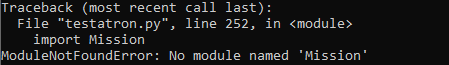
\includegraphics[width=0.7\linewidth]{Testatron_error_without_correct_file_paths.png}}
	\caption{\label{fig:testatron_error}Testatron error without correct file paths.}
\end{figure}

\noindent This error occurs because Testatron needs to be told where your EMTGv9.exe file and PyEMTG directory are if they are not in the default location (``C:\textbackslash emtg\textbackslash bin\textbackslash EMTGv9.exe'' and ``C:\textbackslash emtg\textbackslash PyEMTG\textbackslash{}'' respectively). These can be set on the command line when Testatron is run, or you can change the defaults by editing the testatron.py file directly. This tutorial will focus on the command line approach. To use the command line to set the location of the EMTGv9.exe file, use the ``-e'' or the ``-{}-emtg'' option followed by the path to the executable. To set the location of the PyEMTG directory, use the ``-p'' or ``-{}-pyemtg'' command followed by the path to the folder. For example, the following command would run the unit tests with the correct \ac{EMTG} and PyEMTG locations:

\texttt{python testatron.py --emtg <EMTG\_root\_dir>\textbackslash bin\textbackslash EMTGv9.exe --pyemtg <EMTG\_root\_di\newline\indent r>\textbackslash PyEMTG\textbackslash{} --unit}

\noindent These two options must be set each time Testatron is run unless your EMTGv9.exe and PyEMTG directory are in the default location.

%%%%%%%%%%%%%%%%%%%%%
\subsection{Test Suites}
\label{sec:test_suites}
%%%%%%%%%%%%%%%%%%%%%

While it is most common to run the unit tests, there are a few other sets of tests that can be run. When running Testatron, only one of these sets should be specified. The available options are explained in Table \ref{tab:testatron_options}. Note that examples do not include paths to \ac{EMTG} or PyEMTG for brevity.

\begin{table}[H]
	\begin{small}
		\begin{tabularx}{\linewidth} { >{\arraybackslash} l >{\arraybackslash}p{17em} >{\arraybackslash} X}
			\hline
			Test Type & Option & Explanation \\
			\hline 
			Unit tests & ``-u'' or ``-{}-unit'' & Runs all tests that are not expected to fail. It is recommended to run these tests when adding a new feature to make sure EMTG is still working properly.\newline\newline Ex:\newline \texttt{python testatron.py -u} \\
 			\hline
			Failed tests & ``-{}-failure \textless path-to-failed\_tests.csv\textgreater'' & Reruns all tests in a ``failed\_tests.csv'' file produced by a previous testatron run. Do not include ``failed\_tests.csv'' in the path. You can include multiple paths in a space separated list. \newline\newline Ex:\newline \texttt{python testatron.py --failure output\textbackslash Thu\_Jun\_15\_121445\_2023} \\
 			\hline
			Mission tests & ``-m'' or ``-{}-mission'' & Runs the tests associated with specific missions that used EMTG. (Not available in the public release.)\newline\newline Ex:\newline \texttt{python testatron.py -m} \\
			\hline
			Test cases & ``-c \textless list-of-test-cases\textgreater'' or\newline ``-{}-cases \textless list-of-test-cases\textgreater'' & Runs the test cases specified in the space separated list following the command. This must be the full path to the test and does not include a file extension.\newline\newline Ex:\newline \texttt{python testatron.py -c <EMTG\_root\_dir> \textbackslash testatron\textbackslash tests\textbackslash output\_options\textbackslash output options\_frameICRF <EMTG\_root\_dir>\textbackslash testa tron\textbackslash tests\textbackslash spacecraft\_options\textbackslash spacecraf toptions\_Chemmargin} \\
			\hline
			Test folders & ``-f \textless list-of-folders\textgreater'' or \newline``-{}-folders \textless list-of-folders \textgreater'' & Runs all the test cases in each folder specified in the space separated list of folders following the command.\newline\newline Ex:\newline\texttt{python testatron.py -f global\_mission\_options journey\_options} \\
			\hline
			Update truths & ``-{}-update-truths'' & Replaces the truth cases (*.emtg files) for all tests with the output of this Testatron run. This is useful if an update has caused every test to fail (e.g., a new option has been added).\newline\newline Ex:\newline\texttt{python testatron.py --update-truths} \\
			\hline
			All tests & ``-a'', ``-{}-all'', or none of the above options & Runs all tests, including those in the ``tests\_that\_dont\_work'' folder.\newline\newline Ex:\newline\texttt{python testatron.py -a} or\newline\texttt{python testatron.py} \\
			\hline 
		\end{tabularx} 
	\end{small}
	\caption{\label{tab:testatron_options}Available Testatron test suites.}
\end{table}

%%%%%%%%%%%%%%%%%%%%%
\subsection{Other Options}
\label{sec:other_options}
%%%%%%%%%%%%%%%%%%%%%

You can ignore specific Mission, Journey, or MissionEvent attributes by using the ``-{}-ignore'' option followed by a list of attributes to ignore. Mission attributes should be preceded by ``M.'', Journey attributes by ``J.'', and MissionEvent attributes by ``E.''. When defining this and other lists you should avoid putting them in quotes or brackets and using commas. The list of attributes can be found in the class definitions for Mission, Journey, and MissionEvent. As an example, to run the Testatron unit tests ignoring the chemical\_oxidizer\_used Mission attribute, you can run the command:

\texttt{python testatron.py --emtg <EMTG\_root\_dir>\textbackslash bin\textbackslash EMTGv9.exe --pyemtg <EMTG\_root\_di\newline\indent r>\textbackslash PyEMTG\textbackslash{} --unit --ignore M.chemical\_oxidizer\_used}

%%%%%%%%%%%%%%%%%%%%%
\section{Running Testatron}
\label{sec:running_testatron}
%%%%%%%%%%%%%%%%%%%%%

If you have not already done so, run the Testatron unit tests by running the following command explained in the previous section: 

\texttt{python testatron.py --emtg <EMTG\_root\_dir>\textbackslash bin\textbackslash EMTGv9.exe --pyemtg <EMTG\_root\_di\newline\indent r>\textbackslash PyEMTG\textbackslash{} --unit}

\noindent Testatron will execute the unit tests, which can take up to half an hour. Do not worry if some errors occur during specific \ac{EMTG} runs. These are most often normal \acs{SPICE} errors and do not indicate a failed test. When Testatron finishes, it will list any failed tests and the path to the test as shown in Figure \ref{fig:testatron_output}. 

\noindent\knownissuelabel{NOTE: The ``solveroptions\_nlp\_skip\_emtg139'' test is currently expected to fail unless the ``-{}-ignore M.number\_of\_solution\_attemps'' argument is utilized.}{known_failing_test}

\begin{figure}[H]
	\centering
	\fbox{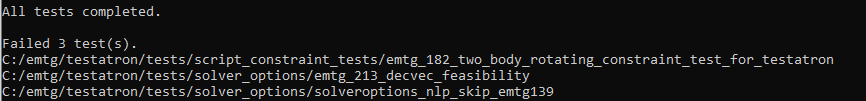
\includegraphics[width=0.9\linewidth]{Testatron_output_from_unit_tests.png}}
	\caption{\label{fig:testatron_output}Testatron output with some failed tests.}
\end{figure}

\newpage
%%%%%%%%%%%%%%%%%%%%%
\section{Output}
\label{sec:output}
%%%%%%%%%%%%%%%%%%%%%

The results from the Testatron run will be located in the \textless EMTG\_root\_dir\textgreater /testatron/output/\textless time-of-test\textgreater{} folder. Where \textless time-of-test\textgreater{} is the date and time the test was run so that each run goes into a separate folder. This folder will contain the *.emtg file from each run of \ac{EMTG}, along with the corresponding *.emtgopt file, and any other files, such as *.emtg\_spacecraftopt files. It also includes the ``failed\_tests.csv'' file and a ``test\_results.csv'' file. The ``failed\_tests.csv'' file lists only the failed tests and the amount of error and tolerance for each test. If a test is listed with no other information, it is likely that the test caused an error while running \ac{EMTG}. As discussed in the Configuration section, the ``failed\_tests.csv'' file can be used with the ``-{}-failure'' option to rerun the failed tests. The ``test\_results.csv'' file lists all the tests that were run and whether they were successful. These files can be used as a starting point to troubleshoot any issues with \ac{EMTG} introduced by new updates.


\end{document}